
\newpage

\begin{tikzpicture}[remember picture,overlay]
  \node[anchor=north west,outer sep=0,inner sep=0] (img) at (current page.north west) {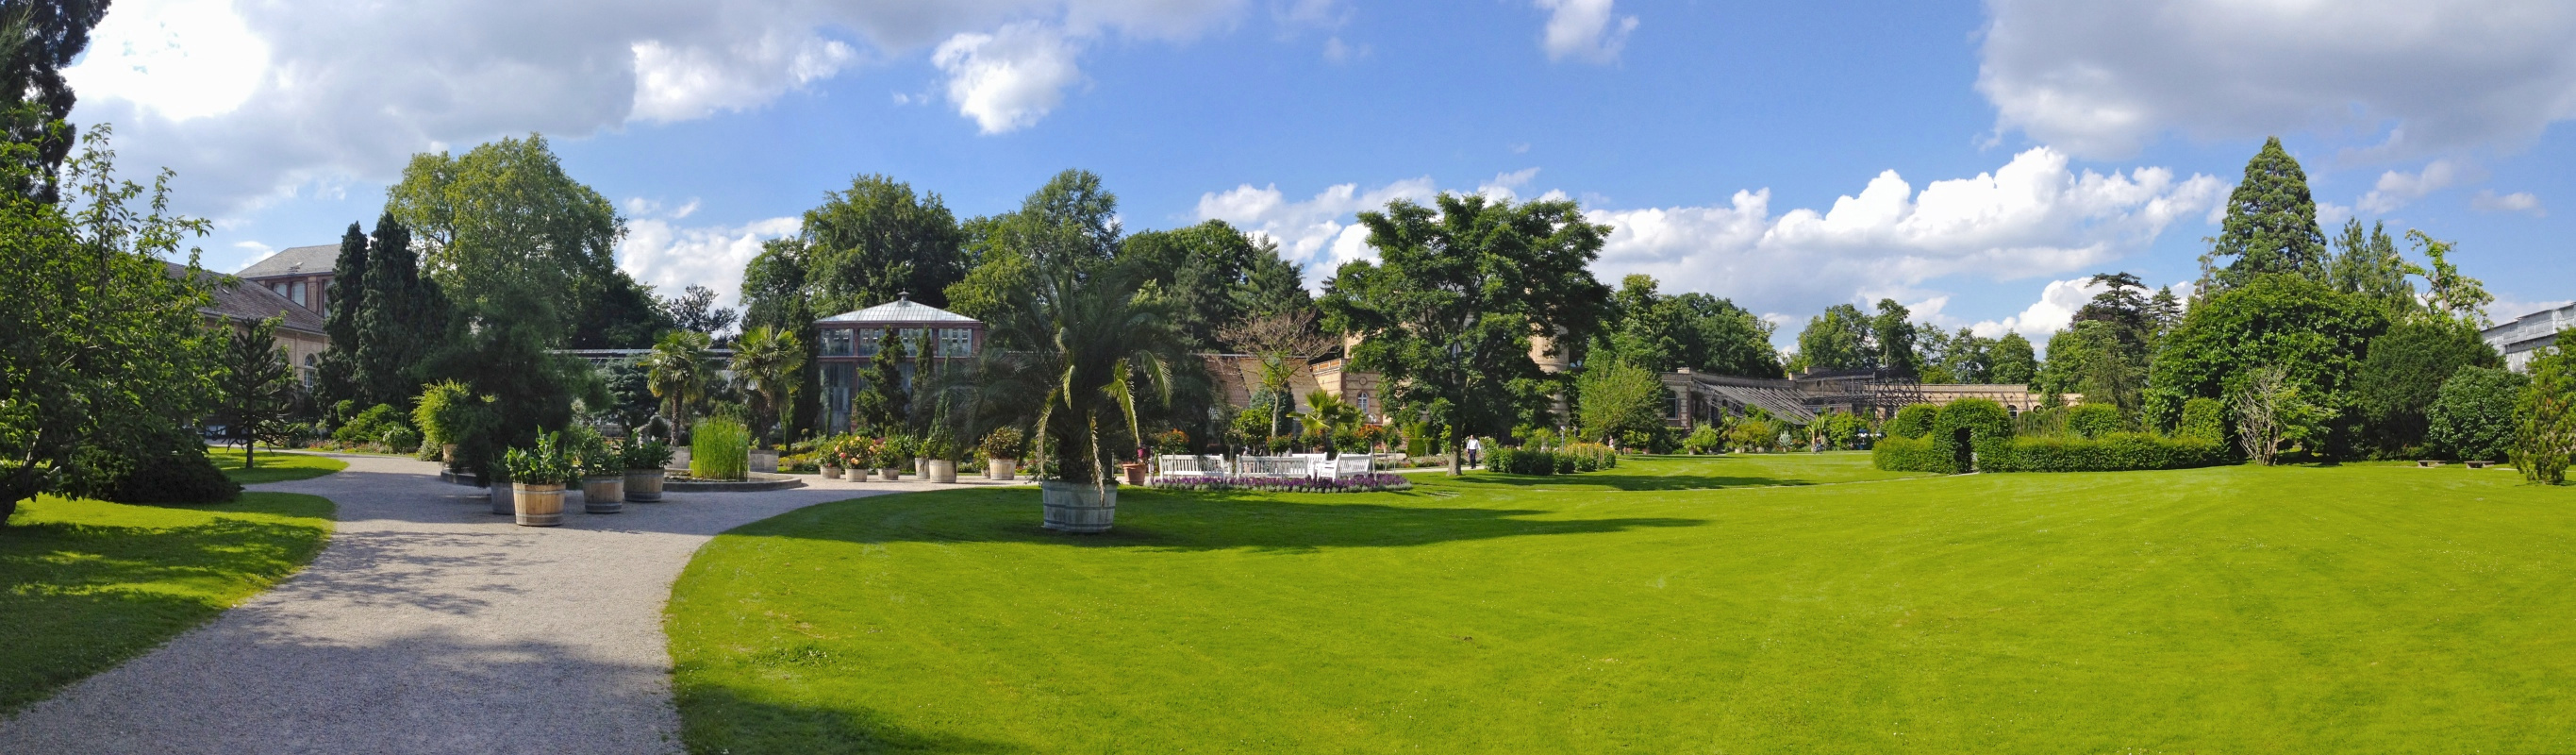
\includegraphics[width=21cm]{images/city/botanic-1.jpg}};
  \node[anchor=south west,outer sep=1ex,color=white] at (img.south west) {\imgtitle{Robin Leffmann}{Botanic Garden}{CC BY-SA 3.0, saturation changed, \url{https://en.wikipedia.org/wiki/File:Karlsruhe_Orangerie_garden_panorama.jpg}}};
\end{tikzpicture}

\vspace*{3.2cm}

\section{Travel}

\subsection{International}

Karlsruhe is a generally well connected city. While it does not have a major
international airport of its own, there are numerous airports well within reach
to allow both overseas and European visitors a cost effective journey. The city
is well connected to the Deutsche Bahn ICE/IC train network and also offers
direct TGV connections to Paris and Marseille (via Lyon). In addition to this
there are numerous far distant bus routes connecting Karlsruhe with destinations
all over Europe.

\begin{multicols}{2}
\raggedcolumns

\subsubsection{Frankfurt Airport (FRA)}

Frankfurt International Airport (FRA) is Germany's busiest airport and an important hub for
international air travel.
\begin{labeling}{\hspace*{10ex}}
  \item[\bf Distance] 130\,km
  \item[\bf By Train] 1\,h, $\SI{40}{\euro}$
  \item[\bf By Bus] \SI{1.5}{h}–\SI{4}{h}, $\ge\SI{10}{\euro}$
\end{labeling}

\subsubsection{Stuttgart Airport (STX)}

About 55 airlines are flying to over a 100 destinations from Stuttgart airport.
It is reachable both by S-Bahn and train or using far distance buses.

\begin{labeling}{\hspace*{10ex}}
  \item[\bf Distance] 80\,km
  \item[\bf By Train] \SI{1.5}{\hour}, $\SI{28}{\euro}$
  \item[\bf By Bus] \SI{1}{\hour}, $\ge\SI{5}{\euro}$
\end{labeling}

\subsubsection{Karlsruhe Baden (FKB)}

Karlsruhe Baden Airpark is a small airport located to the south of the city. It
mostly hosts cheaper airline companies flying to holiday destinations
throughout Europe.

\begin{labeling}{\hspace*{10ex}}
  \item[\bf Distance] 45\,km
  \item[\bf By Bus] \SI{1}{\hour}, $\SI{7.10}{\euro}$
\end{labeling}

\subsubsection{Strasbourg/Entzheim (SXB)}

This airport located just south of Strasbourg can easily be reached from Karlsruhe
using local trains.

\begin{labeling}{\hspace*{10ex}}
  \item[\bf Distance] 105\,km
  \item[\bf By Train] \SI{2}{\hour}, 20 to $\SI{30}{\euro}$
\end{labeling}

\end{multicols}

% There should be a new page here
\newpage


\subsection{Local}

\subsubsection{Walking}
Karlsruhe is a fairly walkable city.
The centre is compact and most things tourists would ever want to visit
are within a 30 minutes stroll.

From the main railway station in the south of the city,
the city's centre is about 25 minute walk.
The university is located right in the centre.
The most promising venue, the DHBW, is a bit off, though.
From the centre, it's another 30 minute walk to the north.
The city is pretty pedestrianised and offers lots of green,
so walking is a pleasure.

\subsubsection{Cycling}
Most local go by bike, though.
Riding the bicycle is very efficient in Karlsruhe and
rental schemes exist.
The most bikes can be had with \href{http://www.faecherrad.de/de/karlsruhe/preise/}{Fächerrad},
which is the localised brand of \href{http://www.nextbike.de/de/news/das-karlsruher-leihfahrrad-hei%C3%9Ft-f%C3%A4cherrad/}{Nextbike},
which is available in many European cities.
So people who are already customers can use those bike right away.
Renting such a bike costs \SI{1}{\euro} per 30 minutes although,
depending on the plan, the first half an hour might be free of charge.

From the main railway station, the city centre is a mere ten minutes 
away.
From the centre to the prospected venue is another ten minutes.



\subsubsection{Public Transport}

Karlsruhe has an efficient public transport system.
It is integrated in the sense that one ticket is valid
for all modes of transport.
So you can go with one ticket by either tram, train, or bus.
The tram from the main railway station takes about 10 minutes.
During rush hours, trams go every five minutes.

The DHBW is connected with a tram which takes 15 minutes to/from the 
main railway station or 10 minutes to/from the centre.
The tram goes every 10 minutes.

The 
\href{http://www.kvv.de/fahrkarten/fahrkarten-preise/einzelfahrkarten.html}%
{prices are as follows}:
A single ride costs \SI{2.40}{\euro}, but you can get four rides for \SI{9.50}{\euro}.
A day pass costs \SI{6.20}{\euro} for one person and \SI{10.10}{\euro} for five 
persons.

\newpage
